%! Author = zarnold
%! Date = 9/20/20

% Preamble
\documentclass{article}

% Packages
\usepackage[english]{babel}
\usepackage[utf8]{inputenc}
\usepackage{amsmath}
\usepackage{amsfonts}
\usepackage{graphicx}
\usepackage{fancyhdr}
\usepackage{tikz}
\usepackage{hyperref}
\usepackage{amssymb}
\pagestyle{fancy}
\graphicspath{ {./images/} }

\fancyhf{}
\rhead{Zach Arnold \linebreak CS 7641 \linebreak Problem Set 1 Answers}
\setlength{\headheight}{52pt}
% Document
\begin{document}
    \section{Question 2 from Problem Set}
    \subsection{Part 1}
    Below is a picture of the inputs and weights (given in the form of $w_1$ and $w_2$), the activation function value is in the
    node with the name $\theta$:
    \linebreak
    \linebreak
    \begin{tikzpicture}[scale=1,auto=center,every node/.style={circle,draw=black!20,thick}]
        \node (a1) at (1,6) {$w_1 = 1/2$};
        \node (a2) at (1,3) {$w_2 = -1/2$};
        \node (a3) at (4,4) {$\theta=3/4$};
        \draw [->] (a1) -- (a3);
        \draw [->] (a2) -- (a3);

    \end{tikzpicture}
    \linebreak
    \linebreak
    For A and B in ${-1, 1}$ we can see the below table:
    \linebreak
    \linebreak
    \begin{tabular}{c c c c}
        $A$ & $B$ & Perceptron Output & Was Activated? \\
        \hline
        -1 & -1 & 0 & False \\
        1 & -1 & 1 & True \\
        -1 & 1 & -1 & False \\
        1 & 1 & 0 & False
    \end{tabular}
    \subsection{Part 2}
    From class lectures we have the following two layered perceptron network:
    \linebreak
    \linebreak
    \begin{tikzpicture}[scale=1,auto=center,every node/.style={circle,draw=black!20,thick}]
        \node (a1) at (1,6) {$w_1 = 1$};
        \node (a2) at (1,3) {$w_2 = 1$};
        \node (a3) at (4,4) {AND $w_3 = -2$};
        \node (a4) at (8,4) {$\theta=1$};

        \draw [->] (a1) -- (a3);
        \draw [->] (a2) -- (a3);
        \draw [->] (a1) -- (a4);
        \draw [->] (a2) -- (a4);
        \draw [->] (a3) -- (a4);

    \end{tikzpicture}
    \linebreak
    \linebreak
    For values of A, B in {0, 1}. Which will produce the following table and verifies that we have achieved XOR function:
    \linebreak
    \linebreak
    \begin{tabular}{c c c c}
        $A$ & $B$ & Perceptron Output & Was Activated? \\
        \hline
        0 & 0 & 0 & False \\
        1 & 0 & 1 & True \\
        0 & 1 & 1 & True \\
        1 & 1 & 0 & False
    \end{tabular}
    \section{Question 5 from Problem Set}
    The piece which makes ID3 Lazy in this context is waiting to construct a tree until the moment a sample needs to be trained.
    \begin{enumerate}
        \item If all attributes of the query record match one record in the training data, then simply return the label otherwise
        \item Remove all records from the training dataset that do not share at least one attribute with the query record
        \item Then perform ID3 like normal to create a decision tree from remaining data (choose the best information gain/split point and construct the tree)
    \end{enumerate}
    Advantages:
    \begin{itemize}
        \item It only considers training examples relevant to query point
        \item Similar to instance based learning methods, Lazy ID3 has no training step and therefore training time is low
        \item No single tree to best generalize for all training examples is constructed therefore this is a flexible algorithm with respect to yet seen data
    \end{itemize}
    Disadvantages:
    \begin{itemize}
        \item Query time is slower since a tree is constructed just in time
        \item It only ever considers examples relevant to the query and likely won't generalize well (overfitting)
    \end{itemize}
    \section{Question 7 from Problem Set}
    \subsection{1, VC Dimension of origin-centered circle}
    An origin centered circle has a VC dimension of 2. The key to answering this is the phrase "origin centered." Since we are not able
    to change the location of the center of the circle then we need to demonstrate that we can shatter two points. Consider
    any two pairs of points $(x_1, y_1), (x_2, y_2) \in {\rm I\!R^2}$ such that $(x_1^2 + y_1^2) \neq (x_2^2 + y_2^2)$.
    That is, thtat they have different radii from the origin. Then it is trivial to show that by varying the radius of the
    circle we can include both points, exclude both points, and separate the two points. As a side note if $(x_1^2 + y_1^2) = (x_2^2 + y_2^2)$
    then the VC dimmension is not two, but one.
    \linebreak
    \linebreak
    \includegraphics[width=10cm, height=10cm]{IMG_0859}
    \linebreak
    My apologies on the lack of origin centeredness, my handwriting is terrible, but hopefully it is clear.
    \subsection{2, VC Dimension of origin-centered sphere}
    An origin centered sphere also has a VC dimension of 2 using similar logic as the above. Becuase we are constrained
    by the fact that this is a perfect sphere (meaning $x^2 + y^2 + z^2 = r^2$ for $x, y, z \in {\rm I\!R^3}$) and by the fact
    that we are centered in the origin (0,0,0), then in fact we can only manipulate the parameter $r^2$ where r is the
    vector from the origin to edge of the sphere. It is impossible to construct a sphere to shatter any 3 points even if they
    are different distances from the origin.

\end{document}